%%%%%%%%%%%%%%%%%%%%%%%%%%%%%%%%%%%%%%%%%
% Beamer Presentation
% LaTeX Template
% Version 1.0 (10/11/12)
%
% This template has been downloaded from:
% http://www.LaTeXTemplates.com
%
% License:
% CC BY-NC-SA 3.0 (http://creativecommons.org/licenses/by-nc-sa/3.0/)
%
%%%%%%%%%%%%%%%%%%%%%%%%%%%%%%%%%%%%%%%%%

%----------------------------------------------------------------------------------------
%	PACKAGES AND THEMES
%----------------------------------------------------------------------------------------

\documentclass[xcolor=table]{beamer}

\mode<presentation> {

% The Beamer class comes with a number of default slide themes
% which change the colors and layouts of slides. Below this is a list
% of all the themes, uncomment each in turn to see what they look like.

%\usetheme{default}
%\usetheme{AnnArbor}
%\usetheme{Antibes}
%\usetheme{Bergen}
%\usetheme{Berkeley}
%\usetheme{Berlin}
%\usetheme{Boadilla}
%\usetheme{CambridgeUS}
%\usetheme{Copenhagen}
%\usetheme{Darmstadt}
%\usetheme{Dresden}
%\usetheme{Frankfurt}
%\usetheme{Goettingen}
%\usetheme{Hannover}
%\usetheme{Ilmenau}
%\usetheme{JuanLesPins}
%\usetheme{Luebeck}
\usetheme{Madrid}
%\usetheme{Malmoe}
%\usetheme{Marburg}
%\usetheme{Montpellier}
%\usetheme{PaloAlto}
%\usetheme{Pittsburgh}
%\usetheme{Rochester}
%\usetheme{Singapore}
%\usetheme{Szeged}
%\usetheme{Warsaw}

% As well as themes, the Beamer class has a number of color themes
% for any slide theme. Uncomment each of these in turn to see how it
% changes the colors of your current slide theme.

%\usecolortheme{albatross}
%\usecolortheme{beaver}
%\usecolortheme{beetle}
%\usecolortheme{crane}
%\usecolortheme{dolphin}
%\usecolortheme{dove}
%\usecolortheme{fly}
%\usecolortheme{lily}
%\usecolortheme{orchid}
%\usecolortheme{rose}
%\usecolortheme{seagull}
%\usecolortheme{seahorse}
%\usecolortheme{whale}
%\usecolortheme{wolverine}

%\setbeamertemplate{footline} % To remove the footer line in all slides 
%%uncomment this line
%\setbeamertemplate{footline}[page number] % To replace the footer line in all 
%%slides with a simple slide count uncomment this line

%\setbeamertemplate{navigation symbols}{} % To remove the navigation symbols 
%%from the bottom of all slides uncomment this line
}

\usepackage{graphicx} % Allows including images
\usepackage{booktabs} % Allows the use of \toprule, \midrule and \bottomrule in 
%tables
\usepackage[french]{babel}
\usepackage{csquotes}
\usepackage{adjustbox}
\usepackage[font=tiny]{subfig}

\usepackage{pgfplots}
\usepgfplotslibrary{fillbetween}
\pgfplotsset{every tick label/.append style={font=\tiny}}

\newcommand\galap[0]{\textsc{G-alap}}
\newcommand\galapllf[0]{\textsc{G-alap-LLF}}
\newcommand\galapedf[0]{\textsc{G-alap-EDF}}
\newcommand\galapezl[0]{\textsc{G-alap-EDZL}}

\setbeamertemplate{navigation symbols}{}

%----------------------------------------------------------------------------------------
%	TITLE PAGE
%----------------------------------------------------------------------------------------

\title[]{Exposé candidature 
Ingénieur d'Études et de Recherche en Systèmes Autonomes} % The short title 
%appears at the 
%bottom of every slide, the full title is only on the title page

\author{Roberto Medina} % Your name
\institute[Inria] % Your institution as it will appear on the bottom of every 
%slide, may be shorthand to save space
{
Post-doctorant dans l'équipe Kopernic, Inria\\
Docteur en informatique de Télécom ParisTech\\
 % Your institution for the title 
%page
\medskip
\textit{roberto.medina-bonilla@inria.fr} % Your email address
}
\date{3 Juillet 2019} % Date, can be changed to a custom date

\begin{document}

\begin{frame}
\titlepage % Print the title page as the first slide
\end{frame}

%----------------------------------------------------------------------------------------
%	PRESENTATION SLIDES
%----------------------------------------------------------------------------------------

\begin{frame}
	\frametitle{Curriculum Vitae}
	\textbf{2015 - Master 2 Recherche} en Informatique - 
			Université Pierre et Marie Curie (Paris 6)
		\begin{itemize}
			\item Spécialité : Systèmes et Applications Distribués.
			\item Stage à Télécom ParisTech : Conception et développement de 
			systèmes critiques sur multi-c\oe{}urs.
		\end{itemize}
	
	\textbf{2019 - Doctorat} en Informatique - Télécom ParisTech
		\begin{itemize}
			\item Déploiement de systèmes à flots de données en criticité mixte 
			pour architectures multi-c\oe{}urs.
			\item Soutenance en Janvier 2019.
			\item \textbf{Assistant d'enseigment} 100h/3ans - élèves 
			ingénieurs/Master/formation continue.
		\end{itemize}
	\textbf{2019 - Post-doctorat} Inria, Équipe Kopernic (Paris)
		\begin{itemize}
			\item Analyse probabiliste des systèmes temps-réel avec contraintes 
			énergétiques.
		\end{itemize}
\end{frame}

%-------------------------------------------------------------------------------

\begin{frame}
	\frametitle{Thème de recherche}
	\centering
	\textbf{Optimisation des techniques d'ordonnancement pour des systèmes 
	embarqués critiques}
	\begin{enumerate}
		\item Criticité mixte sur architectures multi-c\oe{}urs 
		avec tâches dépendantes.
		\begin{itemize}
			\item Calcul de tables d'ordonnancement pour les différents modes 
			d'exécutions du système.
			\item Quantification et amélioration de la disponibilité des tâches 
			moins critiques.
		\end{itemize}
		\item Contraintes énergétiques pour des systèmes temps-réel.
		\begin{itemize}
			\item Mise en évidence des limites des approches existantes.
			\item Adoption des modèles probabilistes pour des techniques de réduction d'énergie.
		\end{itemize}
	\end{enumerate}
\end{frame}

%-------------------------------------------------------------------------------
\section{Ordonnancement à criticité mixte pour tâches dépendantes}
%-------------------------------------------------------------------------------
\subsection{Modèle d'exécution}
%-------------------------------------------------------------------------------

\begin{frame}
	\frametitle{Pire temps d'exécution (WCET)}
	\begin{figure}
		\centering
		\includegraphics<1|handout:0>[width=10cm]{figs/clo0.pdf}
		\includegraphics<2|handout:0>[width=10cm]{figs/clo1.pdf}
		\includegraphics<3|handout:0>[width=10cm]{figs/clo2.pdf}
		\includegraphics<4>[width=10cm]{figs/clo.pdf}
	\end{figure}

	\begin{itemize}
	\item Estimer le WCET : problème très difficile.
		\begin{itemize}
			\item<3-4> Plusieures méthodes possibles pour obtenir une 
			estimation.
			\item<4> Très souvent borné.
			\item<4> Tâches s'exécutent rarement jusqu'au WCET.
			\item<4> Architectures muti-c\oe{}urs peu predictibles.
		\end{itemize}
	\end{itemize}
\end{frame}

%-------------------------------------------------------------------------------

\begin{frame}
	\frametitle{Le modèle à criticité-mixte}
	\begin{enumerate}
		
		\item Incorporer des tâches avec différents niveaux de criticité : HI et LO.
		\item Modes d'exécution :
		\begin{itemize}
			\item Mode LO-criticality : Tâches HI  + tâches LO .
			\item Mode HI-criticality : Tâches HI  $\rightarrow$ Tâches LO dégradées.
		\end{itemize}
		\item Plusieurs pire temps d'exécution.
		\begin{itemize}
			\item $C_i(LO)$: Max. temps d'exécution observé (system designers).
			\item $C_i(HI)$: Borne sup. temps d'exécution (static analysis).
		\end{itemize}
		\item Système passe dans le mode HI-criticality quand c'est nécessaire.
	\end{enumerate}	
\end{frame}

%------------------------------------------------------------------------------

\begin{frame}
	\frametitle{Modèle MC : Ordonnancement avec transition de modes}
	\begin{itemize}
		\item Exemple : tâches HI: $\tau_1, \tau_3$. tâches LO: $\tau_2, \tau_4$.
		\item On assume l'ordonnancement suivant.
		\item<2> Timing Failure Event (TFE) $\rightarrow$ Transition de mode. 
		$\rightarrow$ \textbf{potentiel manque d'échéance}.
	\end{itemize}
	
	\begin{figure}
		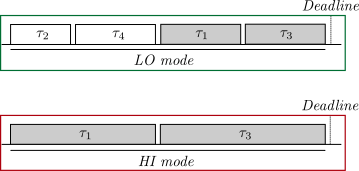
\includegraphics[width=7cm]{figs/mode_transition0}
	\end{figure}
	
	\begin{figure}
		\hspace{1cm}
		\includegraphics<2>[width=8.2cm]{figs/mode_transition}
	\end{figure}
	
\end{frame}

%------------------------------------------------------------------------------

\begin{frame}
	\frametitle{Modèle MC : Disponibilité des tâches LO-criticality}
	\begin{itemize}
		\item Exemple : même lot de tâches d'avant.
	\end{itemize}
	\begin{figure}
		\subfloat{
			\includegraphics<1->[width=7cm]{figs/avail_motiv0.pdf}}
		
		\subfloat{
			\includegraphics<2->[width=7cm]{figs/avail_motiv1.pdf}}
	\end{figure}
	
	\begin{itemize}
		\item<2-> Ordonnançabilité \textit{mais} tâches LO-criticality interrompues :
		ces services ne sont plus disponibles.
	\end{itemize}
\end{frame}

%------------------------------------------------------------------------------
\subsection{DAGs à criticité mixte}
%------------------------------------------------------------------------------

\begin{frame}
	\frametitle{Mixed-Criticality Directed Acyclic Graphs}
	\begin{columns}
		\begin{column}{0.4\textwidth}
			MC-DAG $G \in \mathcal{G}$.\\
			$G=(V, E, D, T)$.
			\begin{itemize}
				\item<2-> $V$ ensemble de n\oe{}uds.
				\item<3-> $E \subseteq (V \times V)$ ensemble d'arcs.
				\item<4-> $D$ échéance.
				\item<5-> $T$ période.
			\end{itemize}
			\only<6->{N\oe{}uds $\tau_i = (\chi_i, 
			C_i(\chi_1), \dots, C_i(\chi_\ell))$}
			\begin{itemize}
				\item<6-> $\chi_i \in \mathcal{CL}$ niveau de criticité.
				\item<7-> $C_i(\chi_1), \dots, C_i(\chi_\ell)$ pire temps d'exécution.
			\end{itemize}
		\end{column}
		\begin{column}{0.6\textwidth}
			\begin{figure}
				\includegraphics<1|handout:0>[width=6cm]{figs/multidag_lo0.pdf}
				\includegraphics<2|handout:0>[width=6cm]{figs/multidag_lo1.pdf}
				\includegraphics<3|handout:0>[width=6cm]{figs/multidag_lo2.pdf}
				\includegraphics<4|handout:0>[width=6cm]{figs/multidag_lo3.pdf}
				\includegraphics<5|handout:0>[width=6cm]{figs/multidag_lo4.pdf}
				\includegraphics<6|handout:0>[width=6cm]{figs/multidag_lo5.pdf}
				\includegraphics<7>[width=6cm]{figs/multidag_lo.pdf}
			\end{figure}
		\end{column}
	\end{columns}
\end{frame}

%-------------------------------------------------------------------------------
%
%\begin{frame}
%	\frametitle{Limites des approches existantes}
%	
%	\begin{alertblock}{Ordonnancement}
%		\begin{itemize}
%			\item Creation de clusters pour ordonnancer des DAGs.
%			\item Généralization à $N$ niveaux.
%		\end{itemize}
%	\end{alertblock}
%	
%	\begin{alertblock}{Disponibilité}
%		\begin{itemize}
%			\item Modèle MC classique interrompt les services moins critiques.
%			\item Rarement reprise de ces services.
%		\end{itemize}
%	\end{alertblock}
%\end{frame}

%------------------------------------------------------------------------------

\begin{frame}
	\frametitle{Problème : ordonnancement MC pour DAGs sur multi-c\oe{}urs}
	\centering
	\begin{itemize}
		\item Ordonnancement pour DAG : problème \textbf{NP-complet}.
		\begin{itemize}
			\item List Scheduling, ordonnanceur TR avec analyse du temps de réponse
			\item \textbf{Pas de variation sur le temps d'exécution} dans la littérature.
			\item \textbf{Pas de transition de modes pour le système}.
		\end{itemize}
		\item<2-> Ordonnancement MC difficile : problème \textbf{NP-difficile}.
		\begin{itemize}
			\item<2-> Majorité des ordonnanceurs (\emph{e.g.} EDF-vd, MC-Fluid) pour lot de tâches 
			\textbf{indépendantes}.
			\item<2-> Quand les contraintes de précédance sont considérées , 
			\textbf{systèmes sont sur-dimensionnés.}
		\end{itemize}
		
	\end{itemize}
	
	\begin{block}{}<3->
		\textbf{Conclusion}: on a besoin de définir des nouvelles méthodes d'ordonnancement efficaces.
	\end{block}
	
\end{frame}

%------------------------------------------------------------------------------
\subsection{Heuristique d'ordonnancement}
%------------------------------------------------------------------------------

\begin{frame}
	\frametitle{Assurer le changement de mode : Safe Transition Property}
	\begin{itemize}
		\item \emph{Intuition}: Pour tout instant $t$, temps d'exécution donné aux tâches HI dans le 
		mode LO, 
		doit être supérieur ou égal au temps d'exécution donné en mode HI.
		\item $\psi_i^{\chi}(t_1, t_2)$: temps d'exécution donné à la tâche $\tau_i$.
	\end{itemize}
	
	\begin{figure}
		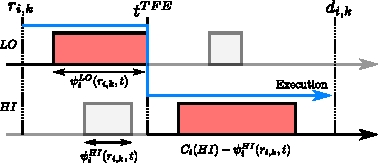
\includegraphics[width=7cm]{figs/proof_case3.pdf}
	\end{figure}
	
	\begin{exampleblock}{Safe Transition Property}
		\begin{equation}
		\psi_i^{LO}(r_{i,k}, t) < C_i(LO) \implies \psi_i^{LO}(r_{i,k}, t) 
		\geq \psi_i^{HI}(r_{i,k},t).
		\label{eq:condswitch}
		\end{equation}
	\end{exampleblock}
\end{frame}

%------------------------------------------------------------------------------

\begin{frame}
	\frametitle{Meta-heuristic for MC-DAG scheduling}
	
	\begin{itemize}
		\item Résoudre le complexe problème d'ordonnancement \emph{hors-ligne} grâce à des 
		\textbf{tables 
		d'ordonnancement}:
		\begin{itemize}
			\item Plus facile à vérifier et à certifier.
			\item Plus facile pour calculer $\psi_i^\chi$, forcer la \textbf{Safe Trans. Prop.}
		\end{itemize}
	\end{itemize}
	
	\begin{exampleblock}{\textsc{Mh-McDag}}
		\begin{itemize}
			\item Calculer la table d'ordonnancement dans le mode HI.
			\item Calculer la table d'ordonnancement dans le mode LO,\\
			en forçant  \textbf{Safe Trans. Prop.}
			\item Changement de mode $\rightarrow$ changement de table d'ordonnancement.
		\end{itemize}
	\end{exampleblock}
\end{frame}

%------------------------------------------------------------------------------

\begin{frame}
	\frametitle{Contraintes sur l'exécution des tâches HI-criticality (1/2)}
	\setcounter{subfigure}{0}
	\begin{itemize}
		\item Approches existantes basés sur des algorithmes à liste (LIst Scheduling).
		\item Calcul de deux ordres de priorité \emph{indépendants}.
		\item Deux tables d'ordonnancement sont produites.
		\item Tâches HI-criticality ordonnancées dès que possible (ASAP).
		\begin{itemize}
			\item Assurer la transition de mode.
		\end{itemize}
		\item Implémentation implicite de \textsc{Mh-McDAG}.
	\end{itemize}
	
\end{frame}

%------------------------------------------------------------------------------

\begin{frame}
	\frametitle{Contraintes sur l'exécution des tâches HI-criticality (2/2)}
	
	\begin{figure}
		\vspace{-0.5cm}
		\begin{tabular}{cc}
			\adjustbox{valign=c}{\subfloat[Single MC-DAG system]{
					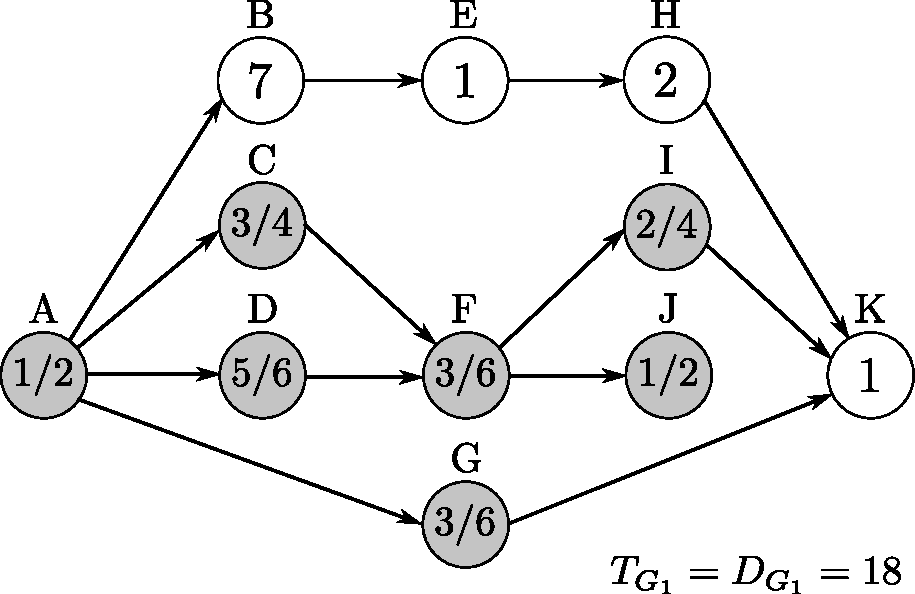
\includegraphics[width=5cm]{figs/ada_lo.pdf}
				}
			}
			
			&
			
			\adjustbox{valign=c}{\begin{tabular}{@{}c@{}}
					\subfloat[$S_{HI}$ scheduling 
					table]{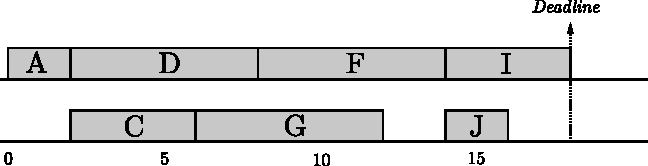
\includegraphics[width=5cm]{figs/ada_baruah_shi.pdf}
						\label{subfig:sched_baruah_shi}}\\
					
					\subfloat[$S_{LO}$ scheduling 
					table]{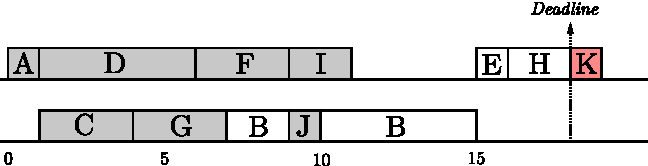
\includegraphics[width=5cm]{figs/ada_baruah_slo.pdf}
						\label{subfig:sched_baruah_slo}}
					\label{fig:sched_baruah_single}
			\end{tabular}}
		\end{tabular}
		
	\end{figure}
	
	\begin{figure}
		\centering
		
	\end{figure}
	
	\begin{alertblock}{}
		\begin{itemize}
			\item Non-ordonnançable avec 18 TUs et 2 c\oe{}urs.
			\item Tâche $B$ prête à être exécutée après 1 TU, constamment preemptée.
			\begin{itemize}
				\item Temps de réponse des tâches LO-criticality affecté.
			\end{itemize}
		\end{itemize}
	\end{alertblock}
	
\end{frame}

%------------------------------------------------------------------------------

\begin{frame}
	\frametitle{Relaxation des tâches HI-criticality (1/2)}
	\begin{itemize}
		
		\item \emph{Exécution au plus tard (ALAP)} des tâches HI dans le mode HI.
		\begin{itemize}
			\item Transformer le graphe dans son \emph{dual} et calculer l'ordonnancement.
		\end{itemize}
		
		
	\end{itemize}
	
	
	\begin{figure}
		\vspace{-0.5cm}
		\begin{tabular}{cc}
			\adjustbox{valign=c}{\subfloat{
					\includegraphics<1|handout:0>[width=5cm]{figs/ada_hi_star0.pdf}
					\includegraphics<2->[width=5cm]{figs/ada_hi_star.pdf}
				}
			}
			
			&
			
			\adjustbox{valign=c}{\begin{tabular}{@{}c@{}}
					\subfloat{
						\includegraphics<3->[width=5cm]{figs/ada_us_shi0.pdf}
					} \\
					
					\subfloat{
						\includegraphics<4->[width=5cm]{figs/ada_us_shi.pdf}
					}
			\end{tabular}}
		\end{tabular}
		
	\end{figure}
\end{frame}

%------------------------------------------------------------------------------

\begin{frame}
	\frametitle{Relaxation des tâches HI-criticality  (2/2)}
	\begin{itemize}
		\item \emph{Prioritization plus précise}: tâches HI-criticality preemptent pour respecter 
		\textbf{Safe Trans. Prop.}
	\end{itemize}
	
	\setcounter{subfigure}{0}
	
	
	\begin{figure}
		\vspace{-0.5cm}
		\begin{tabular}{cc}
			\adjustbox{valign=c}{\subfloat[Single MC-DAG system]{
					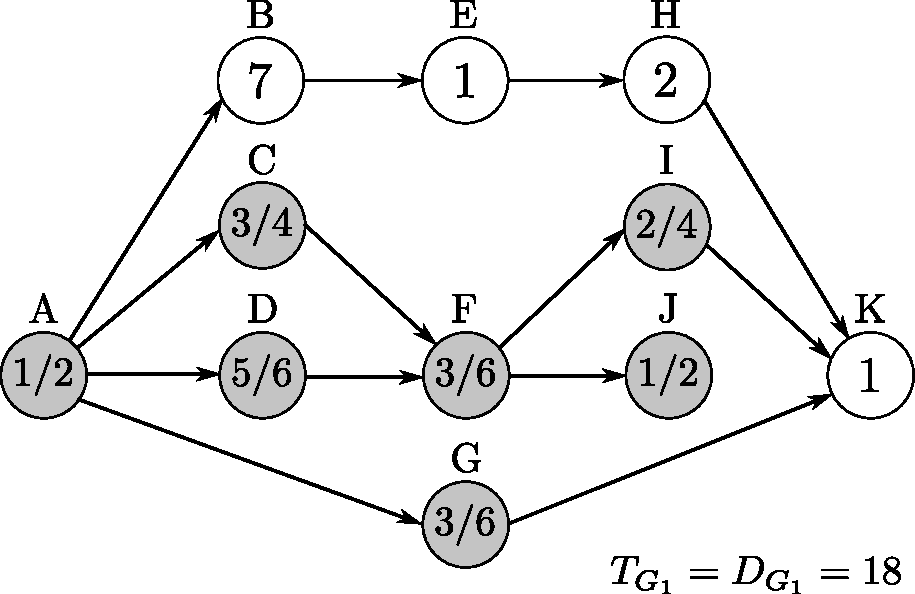
\includegraphics[width=5cm]{figs/ada_lo.pdf}
				}
			}
			
			&
			
			\adjustbox{valign=c}{\begin{tabular}{@{}c@{}}
					\subfloat[ALAP scheduling in HI mode]{
						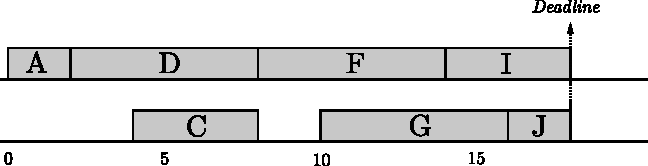
\includegraphics[width=5cm]{figs/ada_us_shi.pdf}} \\
					
					\subfloat[ASAP scheduling in LO mode]{
						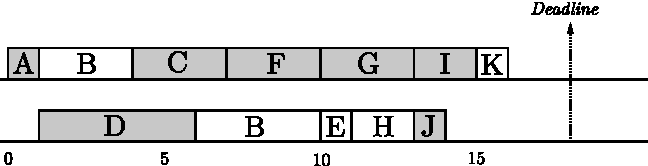
\includegraphics[width=5cm]{figs/ada_us_slo.pdf}}
			\end{tabular}}
		\end{tabular}
		
	\end{figure}
	
	
	\begin{itemize}
		\item Tâches LO-criticality ont plus de timeslots utilisables.
	\end{itemize}
\end{frame}

%------------------------------------------------------------------------------
\subsection {Ordonnancement global multi-périodique}
%------------------------------------------------------------------------------
\newcommand{\light}[1]{\textcolor{gray}{#1}}

\begin{frame}
	\frametitle{MC-DAG multi-périodique}
	Approche existante:
	\begin{itemize}
		\item Fédéré: MC-DAGs catégorisés comme \emph{light} ou \emph{heavy}.
		\begin{itemize}
			\item DAGs light transformés en tâches séquentielles.
			\item DAGs heavy, $U_{max} > 1$, nécessite plus d'un c\oe{}ur pour s'exécuter.
		\end{itemize}
		\item Clusters pour ordonnancer des MC-DAGs heavy sporadiques.
		\item Tables d'ordonnancement calculées pour chaque cluster.
		\item \textbf{Mauvaise gestion des ressources}: n\oe{}uds de MC-DAGs différents ne peuvent pas 
		partager des c\oe{}urs.
	\end{itemize}
\end{frame}

%------------------------------------------------------------------------------

\begin{frame}
	\frametitle{Un exemple de systèmes MC multi-périodique}
	\setcounter{subfigure}{0}
	
	\begin{figure}
		\vspace{-0.7cm}
		\begin{tabular}{cc}
			\adjustbox{valign=c}{\subfloat[MCS multi-périodique]{
					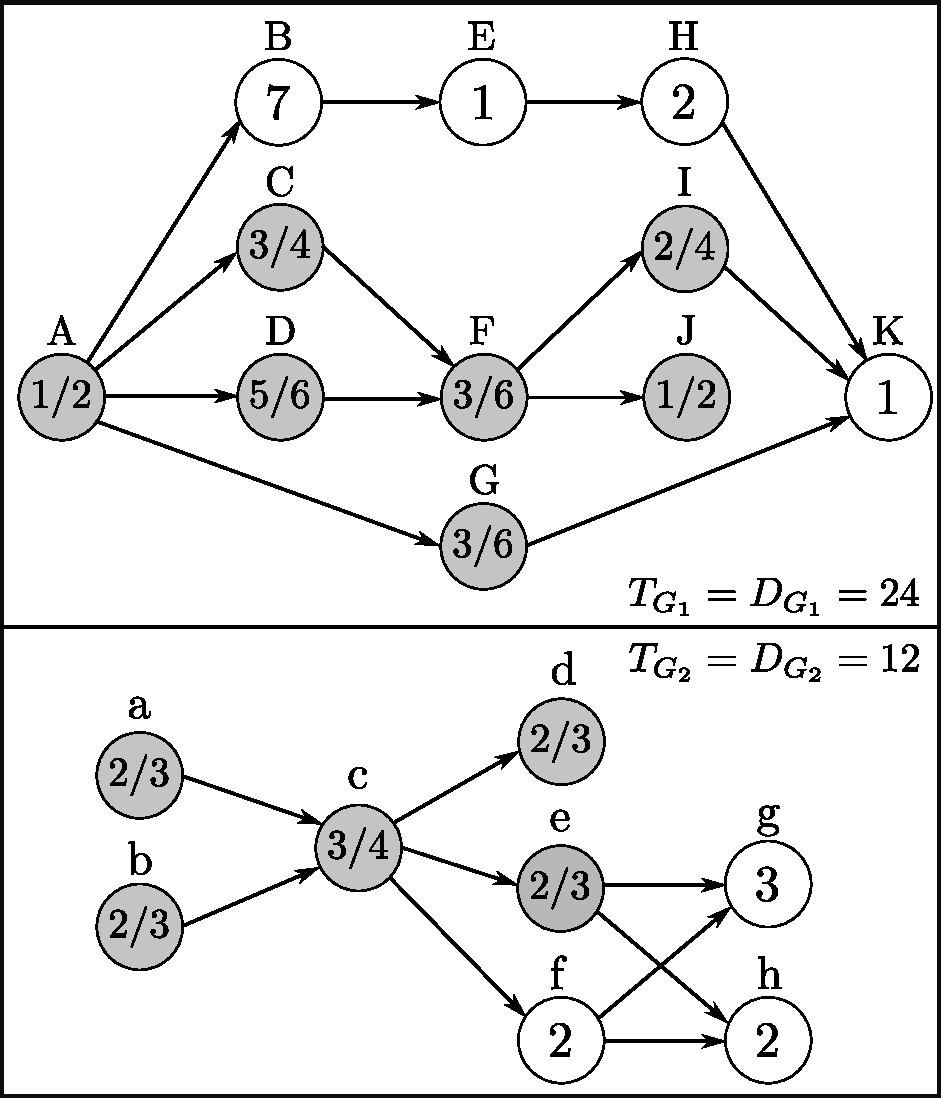
\includegraphics[width=5cm]{figs/multidag_lo.pdf}}}
			
			&
			
			\adjustbox{valign=c}{\begin{tabular}{@{}c@{}}
					\subfloat[Approche fédérée : mode HI-criticality]{
						
						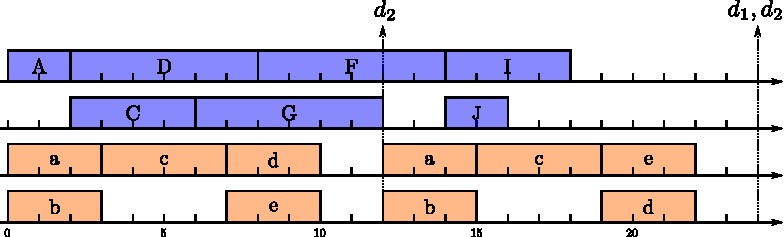
\includegraphics[width=5.5cm]{figs/multiple_shi_federated.pdf}
						\label{subfig:sched_federated_shi}
					}\\
					
					\subfloat[Approche fédérée : mode LO-criticality]{
						
						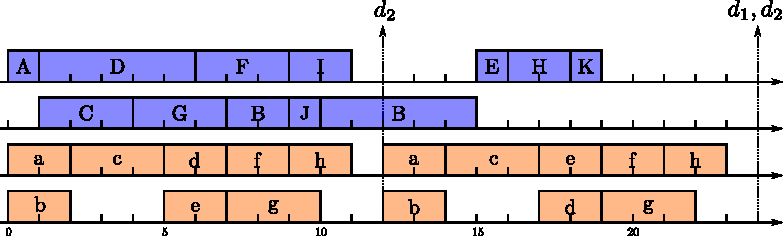
\includegraphics[width=5.5cm]{figs/multiple_slo_federated.pdf}
						\label{subfig:sched_federated_slo}
					}
			\end{tabular}}
		\end{tabular}
	\end{figure}
	
	\begin{itemize}
		\item Au minimum 2 clusters de 2 c\oe{}urs.
		\item Utilisation maximale du système inférieure à 3.
	\end{itemize}
\end{frame}

%------------------------------------------------------------------------------

\begin{frame}
	\frametitle{Approche globale pour MC-DAGs multi-périodiques}
	
	\begin{itemize}
		\item \textbf{Safe Trans. Prop.} utilisable dans le cas multi-périodique.
		\item Plusieurs implémentations possibles grâce à la \textbf{généricité} de \textsc{Mh-McDag}.
	\end{itemize}
	
	\begin{table}
		\begin{tabular}{|c|c|}
			\hline
			\textbf{Implémentation} & \textbf{Ordre de priorité}                                           \\ \hline
			G-EDF                   & $D_{i,k}^\chi = d_{i,k} - 
			CP_i^{\chi}$                            \\ \hline
			G-LLF                   & $L_{i,k}^\chi (t) = d_{i,k} - t - 
			(CP_i^{\chi} + R_{i,k}^{\chi})$ \\ \hline
			Hybrid                  & G-EDF HI mode/G-LLF LO 
			mode                                      \\ \hline
		\end{tabular}
	\end{table}
	%
	%	\begin{itemize}
	%		\item $d_{i,k}$ deadline of the $k$-th activation of the MC-DAG.
	%		\item $CP_i^{\chi}$ critical path to the vertex.
	%		\item $t$ current time slot.
	%		\item $R_{i,k}^{\chi}$ remaining execution time.
	%		\begin{itemize}
	%			\item Initialized with $C_i(LO)$ or $C_i(HI)$.
	%		\end{itemize}Various implementations thanks to
	%	\end{itemize}
	
\end{frame}


%------------------------------------------------------------------------------

\begin{frame}
	\frametitle{\textsc{G-alap} : tables d'ordonnancement}
	\begin{columns}
		\begin{column}{.5\textwidth}
			\begin{figure}
				\centering
				\subfloat[\textsc{G-alap-edf} HI mode]{
					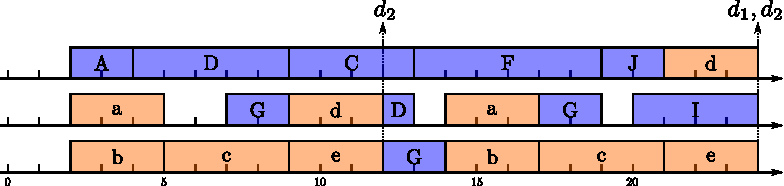
\includegraphics[width=5.5cm]{figs/multiple_shi_edf.pdf}
					\label{subfig:multiple_gedf_hi}
				}
				
				\subfloat[\textsc{G-alap-edf} LO mode]{
					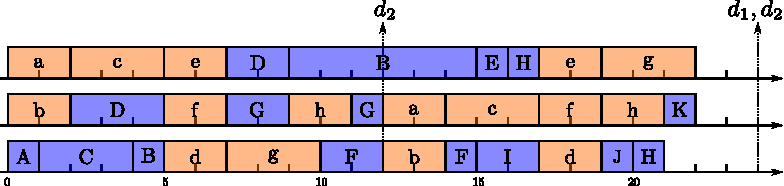
\includegraphics[width=5.5cm]{figs/multiple_slo_edf.pdf}
					\label{subfig:multiple_gedf_lo}
				}
			\end{figure}
		\end{column}
		
		\begin{column}{.5\textwidth}
			\begin{figure}
				
				\subfloat[\textsc{G-alap-llf} HI mode]{
					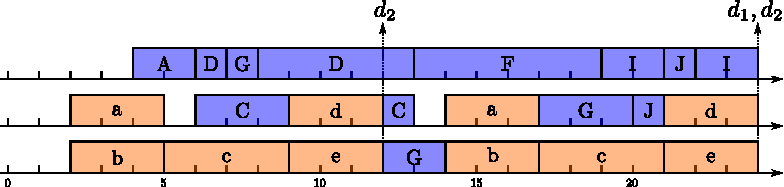
\includegraphics[width=5.5cm]{figs/multiple_shi.pdf}
					\label{subfig:multiple_gllf_hi}
				}
				
				\subfloat[\textsc{G-alap-llf} LO mode]{
					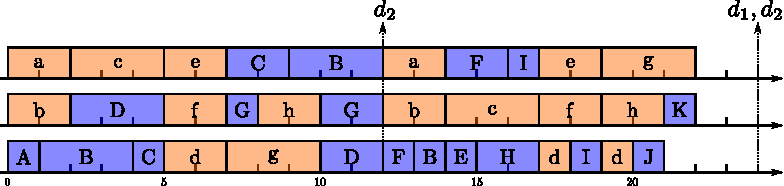
\includegraphics[width=5.5cm]{figs/multiple_slo.pdf}		
					
					\label{fig:multiple_slo}
				}
				
			\end{figure}
		\end{column}
	\end{columns}
	
	
	\begin{itemize}
		\item Tables d'ordonnancement sur \textbf{ 3 c\oe{}urs seulement}.
		\item Ordonnancement MC-DAG multi-périodique efficace.
	\end{itemize}
\end{frame}

%------------------------------------------------------------------------------
\subsection{Niveaux de criticité multiple}
%------------------------------------------------------------------------------

\begin{frame}
	\frametitle{Généralisation de la Safe Transition Property}
	
	\begin{itemize}
		\item \textbf{Problème}: Nécessite calculer plus de tables d'ordonnancement.
	\end{itemize}
	
	\begin{exampleblock}{Safe Transition Property Généralisée}
		\begin{equation}
		\psi_i^{\chi_\ell} (r_{i,k}, t) < C_i(\chi_\ell) \implies 
		\psi_i^{\chi_\ell}(r_{i,k}, t) \geq 
		\psi_i^{\chi_{\ell+1}}(r_{i,k},t).
		\label{eq:start_n_mode_lo}
		\end{equation}
	\end{exampleblock}
	
	\begin{exampleblock}{\textsc{GMH-McDag}}
		Méta-heuristique pour ordonanncement MC-DAG multi-périodique  avec nombre arbitraire de 
		niveaux de criticité.
		\begin{enumerate}
			\item Ordonnancer le système en ordre décroissant.
			\item Pour tous les niveaux de criticité, forcer la \textbf{Safe Trans. Prop. généralisée}.
		\end{enumerate}
	\end{exampleblock}
\end{frame}

%------------------------------------------------------------------------------
\section{Évaluation empirique}
%------------------------------------------------------------------------------
\subsection{Outil de génération}
%------------------------------------------------------------------------------

\begin{frame}
	\frametitle{Outil de génération non-biaisé}		
	\begin{itemize}
		\item Intègre des concepts de différentes communautés.
		\begin{itemize}
			\item Éviter des formes particulières pour les DAGs :créer des n\oe{}uds par couches.
			\item Distribuer l'utilisation du système de manière uniforme.
		\end{itemize}
		\item Plusieurs paramètre doivent être pris en considération.
		\begin{itemize}
			\item Utilisation du système.
			\item Nombre de MC-DAGs.
			\item Nombre de n\oe{}uds par MC-DAG.
			\item Probabilité d'avoir un arc.
			\item Ratio tâches HI/LO-criticality.
		\end{itemize}
		\item Intégré dans un framework open-source~\footnote{MC-DAG 
			framework - \url{https://github.com/robertoxmed/MC-DAG}}.
	\end{itemize}
\end{frame}

%------------------------------------------------------------------------------

\begin{frame}
	\frametitle{Algorithme de génération non-biaisé}
		\setcounter{subfigure}{0}
	\begin{columns}
		\begin{column}{.6\textwidth}
			\begin{exampleblock}{Générateur MC-DAG}
				\begin{enumerate}
					\item<1-> Distribuer l'utilisation.
					\item<1-> Générer un deadline aléatoire.
					\item<2-> Pour chaque niveau de criticité:
					\begin{itemize}
						\item<3-> \textbf{\textit{Phase de génération des n\oe{}uds}} par couches.
						\item<4-> \textbf{\textit{Intégration des arcs}}.
						\item<5-> \textbf{\textit{Phase de réduction}} atteindre un facteur de réduction.
					\end{itemize}
				\end{enumerate}
			\end{exampleblock}
		\end{column}
		
		\begin{column}{0.4\textwidth}
			\begin{figure}
				\includegraphics<3|handout:0>[width=4.5cm]{figs/random_dag0.pdf}
				\includegraphics<4|handout:0>[width=4.5cm]{figs/random_dag1.pdf}
				\includegraphics<5|handout:0>[width=4.5cm]{figs/random_dag2.pdf}
				\includegraphics<6->[width=4.5cm]{figs/random_dag.pdf}
			\end{figure}
		\end{column}
	\end{columns}
\end{frame}

%------------------------------------------------------------------------------
\subsection{Resultats expérimentaux}
%------------------------------------------------------------------------------

\begin{frame}
	\frametitle{Resultats expérimentaux}
	\framesubtitle{Taux d'acceptation pour systèmes MC synthétiques}
	
	\begin{figure}
		\subfloat[\textsc{G-LLF, $|\mathcal{G}| = 1$}]{
			\begin{tikzpicture}[every mark/.append style={mark size=1pt}]
			\begin{axis}[height=4cm, width=0.35\textwidth,
			legend style={nodes={scale=0.4, transform shape}},
			legend pos=north east,grid,
			log ticks with fixed point,
			ytick={0, 0.1, ..., 1.1},
			xtick={0.2, 0.3, ..., 1.1},
			xmin=0.25,	xmax=1,cycle list name=exotic,
			ymin=0]
			
			\path[name path=axis] (axis cs:0.25,0) -- (axis cs:1,0);
			
			\addplot+[name path=llf2] table [x=Unorm, y=LLF] 
			{data/sched/sched_l2_d1.csv};
			\addplot+[name path=llf4] table [x=Unorm, y=LLF] 
			{data/sched/sched_l4_d1.csv};
			\addplot+[name path=llf5] table [x=Unorm, y=LLF] 
			{data/sched/sched_l5_d1.csv};
			
			\addplot[name path=fedllf2] 	table 	[x=Unorm, y=FEDLLF] 
			{data/sched/sched_l2_d1.csv};
			\addplot+[name path=fedllf4] table [x=Unorm, y=FEDLLF] 
			{data/sched/sched_l4_d1.csv};
			\addplot+[name path=fedllf5] table 	[x=Unorm, y=FEDLLF] 
			{data/sched/sched_l5_d1.csv};
			
			\pgfplotsset{cycle list shift=-6}
			\addplot +[fill opacity=0.5] fill between [of=llf2 and axis];
			\addplot +[fill opacity=0.5] fill between [of=llf4 and axis];
			\addplot +[fill opacity=0.5] fill between [of=llf5 and axis];
			\addplot +[gray,fill opacity=0.5] fill between [of=fedllf2 and axis];
			\addplot +[fill opacity=0.5] fill between [of=fedllf4 and axis];
			\addplot +[fill opacity=0.5] fill between [of=fedllf5 and axis];
			
			\end{axis}
			\end{tikzpicture}
			\label{subfig:acceptance-llf}
		}
		\subfloat[\textsc{G-EDF, $|\mathcal{G}| = 1$}]{
			\begin{tikzpicture}[every mark/.append style={mark size=1.2pt}]
			\begin{axis}[	height=4cm, width=0.35\textwidth,
			legend style={nodes={scale=0.5, transform shape}},
			legend pos=north east,grid,
			log ticks with fixed point,
			ytick={0, 0.1, ..., 1.1},
			xtick={0.2, 0.3, ..., 1.1},
			xmin=0.25,	xmax=1,cycle list name=exotic,
			ymin=0]
			
			\path[name path=axis] (axis cs:0.25,0) -- (axis cs:1,0);
			
			\addplot+[name path=edf2] table [x=Unorm, y=EDF] 
			{data/sched/sched_l2_d1.csv};
			\addplot+[name path=edf4] table [x=Unorm, y=EDF] 
			{data/sched/sched_l4_d1.csv};
			\addplot+[name path=edf5] table [x=Unorm, y=EDF] 
			{data/sched/sched_l5_d1.csv};
			
			\addplot[name path=fededf2] 	table 	[x=Unorm, y=FEDEDF] 
			{data/sched/sched_l2_d1.csv};
			\addplot+[name path=fededf4] table [x=Unorm, y=FEDEDF] 
			{data/sched/sched_l4_d1.csv};
			\addplot+[name path=fededf5] table 	[x=Unorm, y=FEDEDF] 
			{data/sched/sched_l5_d1.csv};
			
			\pgfplotsset{cycle list shift=-6}
			\addplot +[fill opacity=0.5] fill between [of=edf2 and axis];
			\addplot +[fill opacity=0.5] fill between [of=edf4 and axis];
			\addplot +[fill opacity=0.5] fill between [of=edf5 and axis];
			\addplot +[gray,fill opacity=0.5] fill between [of=fededf2 and axis];
			\addplot +[fill opacity=0.5] fill between [of=fededf4 and axis];
			\addplot +[fill opacity=0.5] fill between [of=fededf5 and axis];
			
			\end{axis}
			\end{tikzpicture}
			\label{subfig:acceptance-edf-d1}
		}
		\subfloat[\textsc{G-EDZL, $|\mathcal{G}| = 1$}]{
			\begin{tikzpicture}[every mark/.append style={mark size=1.2pt}]
			\begin{axis}[	height=4cm, width=0.35\textwidth,
			legend style={nodes={scale=0.4, transform shape}},
			legend pos=north east,grid,
			log ticks with fixed point,
			ytick={0, 0.1, ..., 1.1},
			xtick={0.2, 0.3, ..., 1.1},
			xmin=0.25,	xmax=1,cycle list name=exotic,
			ymin=0]
			\path[name path=axis] (axis cs:0.25,0) -- (axis cs:1,0);
			
			\addplot+[name path=ezl2] table [x=Unorm, y=EZL] 
			{data/sched/sched_l2_d1.csv};
			\addplot+[name path=ezl4] table [x=Unorm, y=EZL] 
			{data/sched/sched_l4_d1.csv};
			\addplot+[name path=ezl5] table [x=Unorm, y=EZL] 
			{data/sched/sched_l5_d1.csv};
			
			\addplot[name path=fedezl2] 	table 	[x=Unorm, y=FEDEZL] 
			{data/sched/sched_l2_d1.csv};
			\addplot+[name path=fedezl4] table [x=Unorm, y=FEDEZL] 
			{data/sched/sched_l4_d1.csv};
			\addplot+[name path=fedzl5] table 	[x=Unorm, y=FEDEZL] 
			{data/sched/sched_l5_d1.csv};
			
			\pgfplotsset{cycle list shift=-6}
			\addplot +[fill opacity=0.5] fill between [of=ezl2 and axis];
			\addplot +[fill opacity=0.5] fill between [of=ezl4 and axis];
			\addplot +[fill opacity=0.5] fill between [of=ezl5 and axis];
			\addplot +[gray,fill opacity=0.5] fill between [of=fedezl2 and axis];
			\addplot +[fill opacity=0.5] fill between [of=fedezl4 and axis];
			\addplot +[fill opacity=0.5] fill between [of=fedzl5 and axis];
			
			\end{axis}
			\end{tikzpicture}
			\label{subfig:acceptance-ezl-d1}
		}
	
			\subfloat[\textsc{G-LLF, $|\mathcal{G}| = 2$}]{
				\begin{tikzpicture}[every mark/.append style={mark size=1.2pt}]
				\begin{axis}[	height=4cm, width=0.35\textwidth,
				legend style={nodes={scale=0.4, transform shape}},
				legend pos=north east,grid,
				log ticks with fixed point,
				ytick={0, 0.1, ..., 1.1},
				xtick={0.2, 0.3, ..., 1.1},
				xmin=0.25,	xmax=1,cycle list name=exotic,
				ymin=0]
				\path[name path=axis] (axis cs:0.25,0) -- (axis cs:1,0);
				
				\addplot+[name path=llf2] table [x=Unorm, y=LLF] 
				{data/sched/sched_l2_d2.csv};
				\addplot+[name path=llf4] table [x=Unorm, y=LLF] 
				{data/sched/sched_l4_d2.csv};
				\addplot+[name path=llf5] table [x=Unorm, y=LLF] 
				{data/sched/sched_l5_d2.csv};
				
				\addplot[name path=fedllf2] 	table 	[x=Unorm, y=FEDLLF] 
				{data/sched/sched_l2_d2.csv};
				\addplot+[name path=fedllf4] table [x=Unorm, y=FEDLLF] 
				{data/sched/sched_l4_d2.csv};
				\addplot+[name path=fedllf5] table 	[x=Unorm, y=FEDLLF] 
				{data/sched/sched_l5_d2.csv};
				
				\pgfplotsset{cycle list shift=-6}
				\addplot +[fill opacity=0.5] fill between [of=llf2 and axis];
				\addplot +[fill opacity=0.5] fill between [of=llf4 and axis];
				\addplot +[fill opacity=0.5] fill between [of=llf5 and axis];
				\addplot +[gray,fill opacity=0.5] fill between [of=fedllf2 and axis];
				\addplot +[fill opacity=0.5] fill between [of=fedllf4 and axis];
				\addplot +[fill opacity=0.5] fill between [of=fedllf5 and axis];
				\end{axis}
				\end{tikzpicture}
				\label{subfig:acceptance-llf-d2}
			}
			\subfloat[\textsc{G-EDF, $|\mathcal{G}| = 2$}]{
				\begin{tikzpicture}[every mark/.append style={mark size=1.2pt}]
				\begin{axis}[	height=4cm, width=0.35\textwidth,
				legend style={nodes={scale=0.4, transform shape}},
				legend pos=north east,grid,
				log ticks with fixed point,
				ytick={0, 0.1, ..., 1.1},
				xtick={0.2, 0.3, ..., 1.1},
				xmin=0.25,	xmax=1,cycle list name=exotic,
				ymin=0]
				\path[name path=axis] (axis cs:0.25,0) -- (axis cs:1,0);
				
				\addplot+[name path=edf2] table [x=Unorm, y=EDF] 
				{data/sched/sched_l2_d2.csv};
				\addplot+[name path=edf4] table [x=Unorm, y=EDF] 
				{data/sched/sched_l4_d2.csv};
				\addplot+[name path=edf5] table [x=Unorm, y=EDF] 
				{data/sched/sched_l5_d2.csv};
				
				\addplot[name path=fededf2] 	table 	[x=Unorm, y=FEDEDF] 
				{data/sched/sched_l2_d2.csv};
				\addplot+[name path=fededf4] table [x=Unorm, y=FEDEDF] 
				{data/sched/sched_l4_d2.csv};
				\addplot+[name path=fededf5] table 	[x=Unorm, y=FEDEDF] 
				{data/sched/sched_l5_d2.csv};
				
				\pgfplotsset{cycle list shift=-6}
				\addplot +[fill opacity=0.5] fill between [of=edf2 and axis];
				\addplot +[fill opacity=0.5] fill between [of=edf4 and axis];
				\addplot +[fill opacity=0.5] fill between [of=edf5 and axis];
				\addplot +[gray,fill opacity=0.5] fill between [of=fededf2 and axis];
				\addplot +[fill opacity=0.5] fill between [of=fededf4 and axis];
				\addplot +[fill opacity=0.5] fill between [of=fededf5 and axis];
				\end{axis}
				\end{tikzpicture}
				\label{subfig:acceptance-edf}
			}
			\subfloat[\textsc{G-EDZL, $|\mathcal{G}| = 2$}]{
				\begin{tikzpicture}[every mark/.append style={mark size=1.2pt}]
				\begin{axis}[	height=4cm, width=0.35\textwidth,
				legend style={nodes={scale=0.4, transform shape}},
				legend pos=north east,grid,
				log ticks with fixed point,
				ytick={0, 0.1, ..., 1.1},
				xtick={0.2, 0.3, ..., 1.1},
				xmin=0.25,	xmax=1,cycle list name=exotic,
				ymin=0]
				
				\path[name path=axis] (axis cs:0.25,0) -- (axis cs:1,0);
				
				\addplot+[name path=ezl2] table [x=Unorm, y=EZL] 
				{data/sched/sched_l2_d2.csv};
				\addplot+[name path=ezl4] table [x=Unorm, y=EZL] 
				{data/sched/sched_l4_d2.csv};
				\addplot+[name path=ezl5] table [x=Unorm, y=EZL] 
				{data/sched/sched_l5_d2.csv};
				
				\addplot[name path=fedezl2] 	table 	[x=Unorm, y=FEDEZL] 
				{data/sched/sched_l2_d2.csv};
				\addplot+[name path=fedezl4] table [x=Unorm, y=FEDEZL] 
				{data/sched/sched_l4_d2.csv};
				\addplot+[name path=fedzl5] table 	[x=Unorm, y=FEDEZL] 
				{data/sched/sched_l5_d2.csv};
				
				\pgfplotsset{cycle list shift=-6}
				\addplot +[fill opacity=0.5] fill between [of=ezl2 and axis];
				\addplot +[fill opacity=0.5] fill between [of=ezl4 and axis];
				\addplot +[fill opacity=0.5] fill between [of=ezl5 and axis];
				\addplot +[gray,fill opacity=0.5] fill between [of=fedezl2 and axis];
				\addplot +[fill opacity=0.5] fill between [of=fedezl4 and axis];
				\addplot +[fill opacity=0.5] fill between [of=fedzl5 and axis];
				
				\end{axis}
				\end{tikzpicture}
				\label{subfig:acceptance-ezl-d2}
			}
	\end{figure}
\end{frame}

%-------------------------------------------------------------------------------
\section{Disponibilité pour systèmes MC}
%-------------------------------------------------------------------------------

\begin{frame}
	\frametitle{Problème : Disponibilité dans les systèmes MC}
	
	
	\centering

	\textbf{Criticité mixte et disponibilité}
		\vspace{.5cm}
		\begin{itemize}
			\item \textbf{Modèle Discard MC} meilleurs résultats d'ordonnancement.
			\item Tâches LO-criticality complètement interrompues.
			\item Tâches LO-criticality sont aussi importantes (QoS).
			\item Pas d'évaluation de disponibilité pour tâches dépendantes dans la littérature.
			\begin{itemize}
				\item Difficile de justifier l'applicabilité du modèle MC.
			\end{itemize}
		\end{itemize}
	
\end{frame}

%-------------------------------------------------------------------------------

\begin{frame}
	\frametitle{Quantification : étapes de modélisation}
	
	\begin{enumerate}
		\item Tables d'ordonnancement (grâce à notre méta-heuristique).
		\item<2-> \textbf{Modèle de fautes} : probabilité d'avoir une TFE.
		\item<3-> \textbf{Mécanisme de reprise}: redémarre le mode LO mode après l'hyper-période.
	\end{enumerate}
	
	\begin{columns}
		\begin{column}{.5\textwidth}
			\begin{figure}
				\vspace{-0.5cm}
				\includegraphics<1|handout:0>[width=4cm]{figs/avail_lo0.pdf}
				\includegraphics<2->[width=4cm]{figs/avail_lo1.pdf}
			\end{figure}
		\end{column}
		\begin{column}{.5\textwidth}
			\begin{figure}
				\includegraphics<1-2|handout:0>[width=5cm]{figs/time_empty.pdf}
				\includegraphics<3|handout:0>[width=5cm]{figs/recovery_ex1.pdf}
				\includegraphics<4|handout:0>[width=5cm]{figs/recovery_ex2.pdf}
				\includegraphics<5|handout:0>[width=5cm]{figs/recovery_ex3.pdf}
				\includegraphics<6>[width=5cm]{figs/recovery_ex4.pdf}
			\end{figure}
		\end{column}
	\end{columns}
\end{frame}

%-------------------------------------------------------------------------------

\begin{frame}
	\frametitle{Amélioration de la disponibilité : tâches temps-réel weakly-hard}
	\begin{itemize}
		\item Tolérer un nombre fixe $m$ de fautes sur $k$ exécutions successives.
		\item Comportement d'une tâche WHRT $(1-2)$-firm:
	\end{itemize}
	
	\begin{figure}
		\subfloat{
			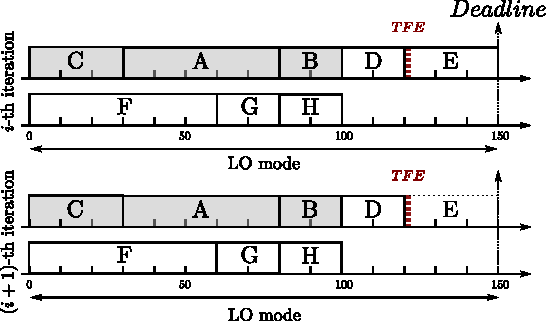
\includegraphics[width=5cm]{figs/mkfirm_time3.pdf}
		}\quad
		\subfloat{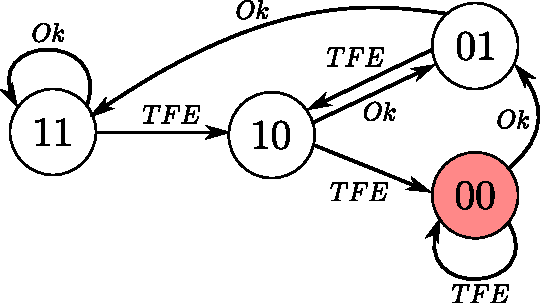
\includegraphics[width=4.5cm]{figs/mkfirm.pdf}}
	\end{figure}
\end{frame}

%-------------------------------------------------------------------------------

\begin{frame}
	\frametitle{Simulations du système : automate probabiliste}
	\centering
	\textbf{Problème:} État courant du système dépend des exécution précédantes 
	executions $\rightarrow$ mémoriser les états précédants.
	\begin{itemize}
		\item<2-> \textbf{Solution}: Règles de transformation vers automate PRISM probabiliste.
		\begin{itemize}
			\item<3-> \textit{Défi 1}: passage à l'échelle.
			\item<3-> \textit{Défi 2}: automatisation.
			
		\end{itemize}
		
	\end{itemize}
	\setcounter{subfigure}{0}
	\begin{figure}
		\vspace{-0.7cm}
		\subfloat{
			\includegraphics<4->[width=3.5cm]{figs/mk_r1.pdf}
			\label{subfig:prism_r1}
		}
		\subfloat{
			\includegraphics<4->[width=3.5cm]{figs/mk_r2.pdf}
			\label{subfig:prism_r2}
		}
		\subfloat{
			\includegraphics<4->[width=3.5cm]{figs/mk_r3.pdf}
			\label{subfig:prism_r3}
		}
		\label{fig:prism_rules}
	\end{figure}
\end{frame}

%------------------------------------------------------------------------------

\begin{frame}
	\frametitle{Simulations du système: résultats}
	
	\begin{figure}
		\subfloat{
			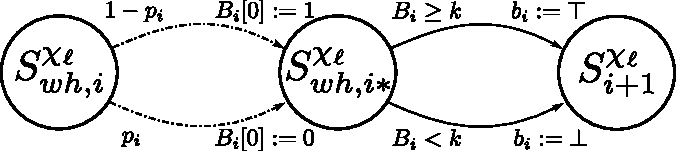
\includegraphics[width=7cm]{figs/mk_r4.pdf}
			\label{subfig:prism_r4}
		}
	\end{figure}
	
	\begin{table}[]	
		\centering
		\begin{tabular}{c|c|c|c|}
			\cline{2-4}
			\multicolumn{1}{l|}{}                  & 
			\multicolumn{3}{c|}{\textbf{Taux de Disponibilité}} \\ \hline
			\multicolumn{1}{|c|}{\textbf{Sorties}} & Discard MC  & Enhanced FP  
			& 
			Enhanced FP + WHRT \\ \hline
			\multicolumn{1}{|c|}{\textit{E}}       & 95.78900\%    & 
			96.98900\%     
			&       \only{\textbf{97.90121\%}}<2->       \\ \hline
			\multicolumn{1}{|c|}{\textit{F}}       & 98.90000\%      & 
			98.90000\%       & 
			\only{98.90099\%}<2->             \\ \hline
			\multicolumn{1}{|c|}{\textit{H}}       & 97.79000\%     & 
			98.89000\%      & \only{98.89441\%}<2->         \\ \hline
		\end{tabular}
		\label{tab:avail_enhance}
	\end{table}
	\begin{itemize}
		\item<2-> Disponibilité évalué par PRISM en PCTL.
		\item<2-> Règles de transformation dans le framework MC-DAG.
	\end{itemize}
\end{frame}

%-------------------------------------------------------------------------------
\section{Consommation énergétique pour systèmes embarqués critiques}
%-------------------------------------------------------------------------------

\begin{frame}
	\frametitle{Problème: Réduction de la consommation énergétique sous contraintes temps-réelles}
	\framesubtitle{Sera présenté à RTSOPS 2019}
	\begin{itemize}
		\item Réduire la fréquence des processeurs pour consommer moins d'énergie ($\searrow$ tension 
		$\rightarrow$ $\searrow$ fréquence)
		\begin{itemize}
			\item Incrémente le temps d'exécution des tâches.
		\end{itemize}
		\item Méthodes Dynamic Voltage and Frequency Scaling (DVFS) existantes ont deux limites majeures:
		\begin{enumerate}
			\item Temps d'exécution d'une tâche proportionnel à la fréquence du processeur.
			\item Réduction énergétique uniquement au niveau du processeur, autres composants (mémoire, 
			périphériques) ignorés.
		\end{enumerate}
	\end{itemize}
	
\end{frame}

\begin{frame}
	\frametitle{Évolution du nombre de cycles sous différentes fréquences}
	\centering
	\includegraphics[width=12cm]{figs/cycles.png}
	\vspace{-.5cm}
	\begin{itemize}
		\item Temps d'exécution pas exactement proportionnel $\rightarrow$ mémoire goulot d'étranglement.
	\end{itemize}
\end{frame}


%-------------------------------------------------------------------------------
\begin{frame}
	\frametitle{Publications \& Valorisation}
	\begin{table}[]
		\begin{tabular}{|l|c|l|}
			\hline
			\rowcolor[HTML]{DAE8FC} 
			Total                      & 7          &                          \\ \hline
			Journaux                   & \textit{1} & IEEE Trans. on Computers \\ \hline
			Conférences (Papiers)      & 3          & RTSS, DATE, Ada Europe   \\ \hline
			Conférences (WIP + Poster) & \textit{2} & RTSS, SIES               \\ \hline
			Thèse                      & 1          &                          \\ \hline
		\end{tabular}
	\end{table}
	\textbf{Séminaires externes et diffusion de l'information scientifique}
	\begin{itemize}
        \item INRIA, Rennes, 2017, Scheduling of DAGs for mixed-criticality systems.
		\item INRIA, Paris, 2018, Scheduling and availability analysis for DAGs on 
		mixed-criticality systems.
		\item CEA List, Palaiseau, 2018, Scheduling of multi-periodic DAGs on 
		multi-core for mixed-criticality.
		\item T\'{e}l\'{e}com ParisTech, 2018, ``Journ\'{e}es Recherche du LTCI''.
	\end{itemize}
\end{frame}

%-------------------------------------------------------------------------------
\section{Projet de recherche}

%-------------------------------------------------------------------------------
\begin{frame}
	\frametitle{Integration DTIS/SEAS: projet de recherche}
	
	\begin{itemize}
		\item \textbf{Contexte équipe :}
		\begin{itemize}
			\item Spécification, conception, développement et analyse de systèmes autonomes.
		\end{itemize}
		\item \textbf{Proposition:}
		\begin{itemize}
			\item Spécification et vérification sous contraintes temps-réelles et non-fonctionnelles pour systèmes 
			embarqués autonomes.
		\end{itemize}
	\end{itemize}
	\begin{columns}
		\begin{column}{.45\textwidth}
			\textbf{Thème 1 :}  Spécification, analyse et améliorations des contraintes temps-réelles.
			\begin{itemize}
				\item Analyse temporelle formelle et expérimentale pour architecture robotique.
				\item Développement/amélioration des outils TR sur systèmes robotiques.
			\end{itemize}
		\end{column}
		\begin{column}{.45\textwidth}
			\textbf{Thème 2 :} Contraintes non-fonctionnelles dans la prise de décision de systèmes autonomes.
			\begin{itemize}
				\item Plans d'exécution avec contraintes énergétiques.
			\end{itemize}
		\end{column}
	\end{columns}
	
\end{frame}

%-------------------------------------------------------------------------------
\begin{frame}
	\frametitle{Integration DTIS/SEAS: compétences}
		
	\begin{displayquote}
		\begin{itemize}
			\item \textcolor[rgb]{0.2,0.5,0.2}{Formal specification languages}
			\item \textcolor[rgb]{0.2,0.5,0.2}{Languages for modeling system architectures or their behavior}
			\item \textcolor[rgb]{0.2,0.5,0.2}{Formal verification} or \textcolor[rgb]{0.2,0.5,0.2}{real-time 
			analysis techniques}
			\item Architectures and algorithms for decision-making, from task planning to execution management
			\item Decision-making and multi-machine mission management architectures, distributed between 
			ground stations and onboard systems
			\item \textcolor[rgb]{0.2,0.5,0.2}{Tools and methods for installation on physical platforms}
		\end{itemize}
	\end{displayquote}

	Repris du site \url{https://www.onera.fr/en/dtis/research-units}
	
\end{frame}

%-------------------------------------------------------------------------------
\begin{frame}
	\frametitle{Bilan de candidature}
	
	\begin{itemize}
		\item \textbf{Compétences complémentaires}
		\begin{itemize}
			\item Ordonnancements temps-réels sous différents modèles d'exécution (criticité mixte, 
			DVFS).
			\item Connaissances en méthodes formelles et simulations des systèmes temps-réels.
		\end{itemize}
		\item \textbf{Expérience de recherche}
		\begin{itemize}
			\item Intégration rapide à différentes équipes de recherche sous des objectifs de différents.
			\item Travaux validés dans des conférences internationales importantes.
			\item Recherche dans un cadre industriel : chaire systèmes complexes TPT.
		\end{itemize}
	\end{itemize}
\end{frame}

\end{document} 